\documentclass[25pt, a0paper, portrait, margin=0mm, innermargin=15mm, blockverticalspace=15mm,
  colspace=15mm, subcolspace=8mm]{tikzposter}
\usepackage{DejaVuSans}
\renewcommand{\familydefault}{\sfdefault}
\usepackage{booktabs}
\usepackage{array}
\usepackage{qrcode}
\usetikzlibrary{positioning,arrows.meta}
\newcolumntype{L}[1]{>{\raggedright\arraybackslash}p{#1}}

% FOSDEM 2027's colours; its logo comes from `make art`.
\definecolor{fosdem}{HTML}{AC1D94}
\definecolor{ink}{HTML}{222222}
\definecolor{paper}{HTML}{F6F6F6}
\definecolorstyle{Fosdem}{
  \colorlet{colorOne}{fosdem}\colorlet{colorTwo}{ink}\colorlet{colorThree}{paper}
}{
  \colorlet{backgroundcolor}{white}\colorlet{framecolor}{white}
  \colorlet{titlefgcolor}{ink}\colorlet{titlebgcolor}{white}
  \colorlet{blocktitlebgcolor}{fosdem}\colorlet{blocktitlefgcolor}{white}
  \colorlet{blockbodybgcolor}{paper}\colorlet{blockbodyfgcolor}{ink}
  \colorlet{innerblocktitlebgcolor}{white}\colorlet{innerblocktitlefgcolor}{ink}
  \colorlet{innerblockbodybgcolor}{white}\colorlet{innerblockbodyfgcolor}{ink}
  \colorlet{notefgcolor}{ink}\colorlet{notebgcolor}{white}\colorlet{noteframecolor}{fosdem}
}
\definetitlestyle{Gear}{width=\paperwidth, roundedcorners=0, linewidth=0pt, innersep=4cm,
  titletotopverticalspace=0mm, titletoblockverticalspace=15mm}{
  \fill[fosdem] (\titleposleft, \titleposbottom) rectangle (\titleposright, \titleposbottom + 1.2cm);
  \IfFileExists{build/art/fosdem.pdf}{\node[anchor=west, inner sep=0] at (\titleposleft + 4cm, 0.5*\titlepostop + 0.5*\titleposbottom + 0.6cm)
    {\includegraphics[height=12cm]{build/art/fosdem.pdf}};}{}}
\usetheme{Simple}
\useblockstyle{Default}
\usetitlestyle{Gear}
\makeatletter
\renewcommand{\TP@maketitle}{\hspace*{15cm}\begin{minipage}{54cm}\raggedright\color{titlefgcolor}
  {\bfseries\Huge\@title\par}\vspace*{0.5em}{\huge with a Mesa Vulkan driver and a Rust DRM driver\par}\vspace*{1em}{\huge\@author\par}\vspace*{0.4em}{\LARGE\color{fosdem}\@institute}\end{minipage}}
\makeatother
\tikzposterlatexaffectionproofoff
\usecolorstyle{Fosdem}
\newcommand{\pblock}[2]{\block{#1}{\Large\raggedright #2}}
\newcommand{\photo}[1]{\fbox{\parbox[c][17cm]{0.9\linewidth}{\centering\textit{photo: #1}}}}

\title{Borg: An Open GPU}
\author{Andreas Wendleder}
\institute{github.com/gonsolo/Borg \quad FOSDEM 2027}

\begin{document}
\maketitle

\pblock{}{
  \begin{minipage}[c]{0.5\linewidth}
    \Large A GPU you can read end to end, and every layer above it open too: the GPU in Chisel, a
    64-bit RISC-V CPU that boots Linux, a Rust DRM/KMS driver in the kernel, and a native Mesa
    Vulkan driver in Rust with its own shader compiler.\\[5mm]
    \textbf{Running here:} the unmodified Khronos \texttt{vkcube} under Linux on the board,
    rendered by Borg, on HDMI.
  \end{minipage}\hfill
  \begin{minipage}[c]{0.46\linewidth}
    \centering\photo{the Nexys Video, vkcube full screen over HDMI}
  \end{minipage}
}

\begin{columns}
\column{0.333}
\pblock{The whole stack}{
  \centering
  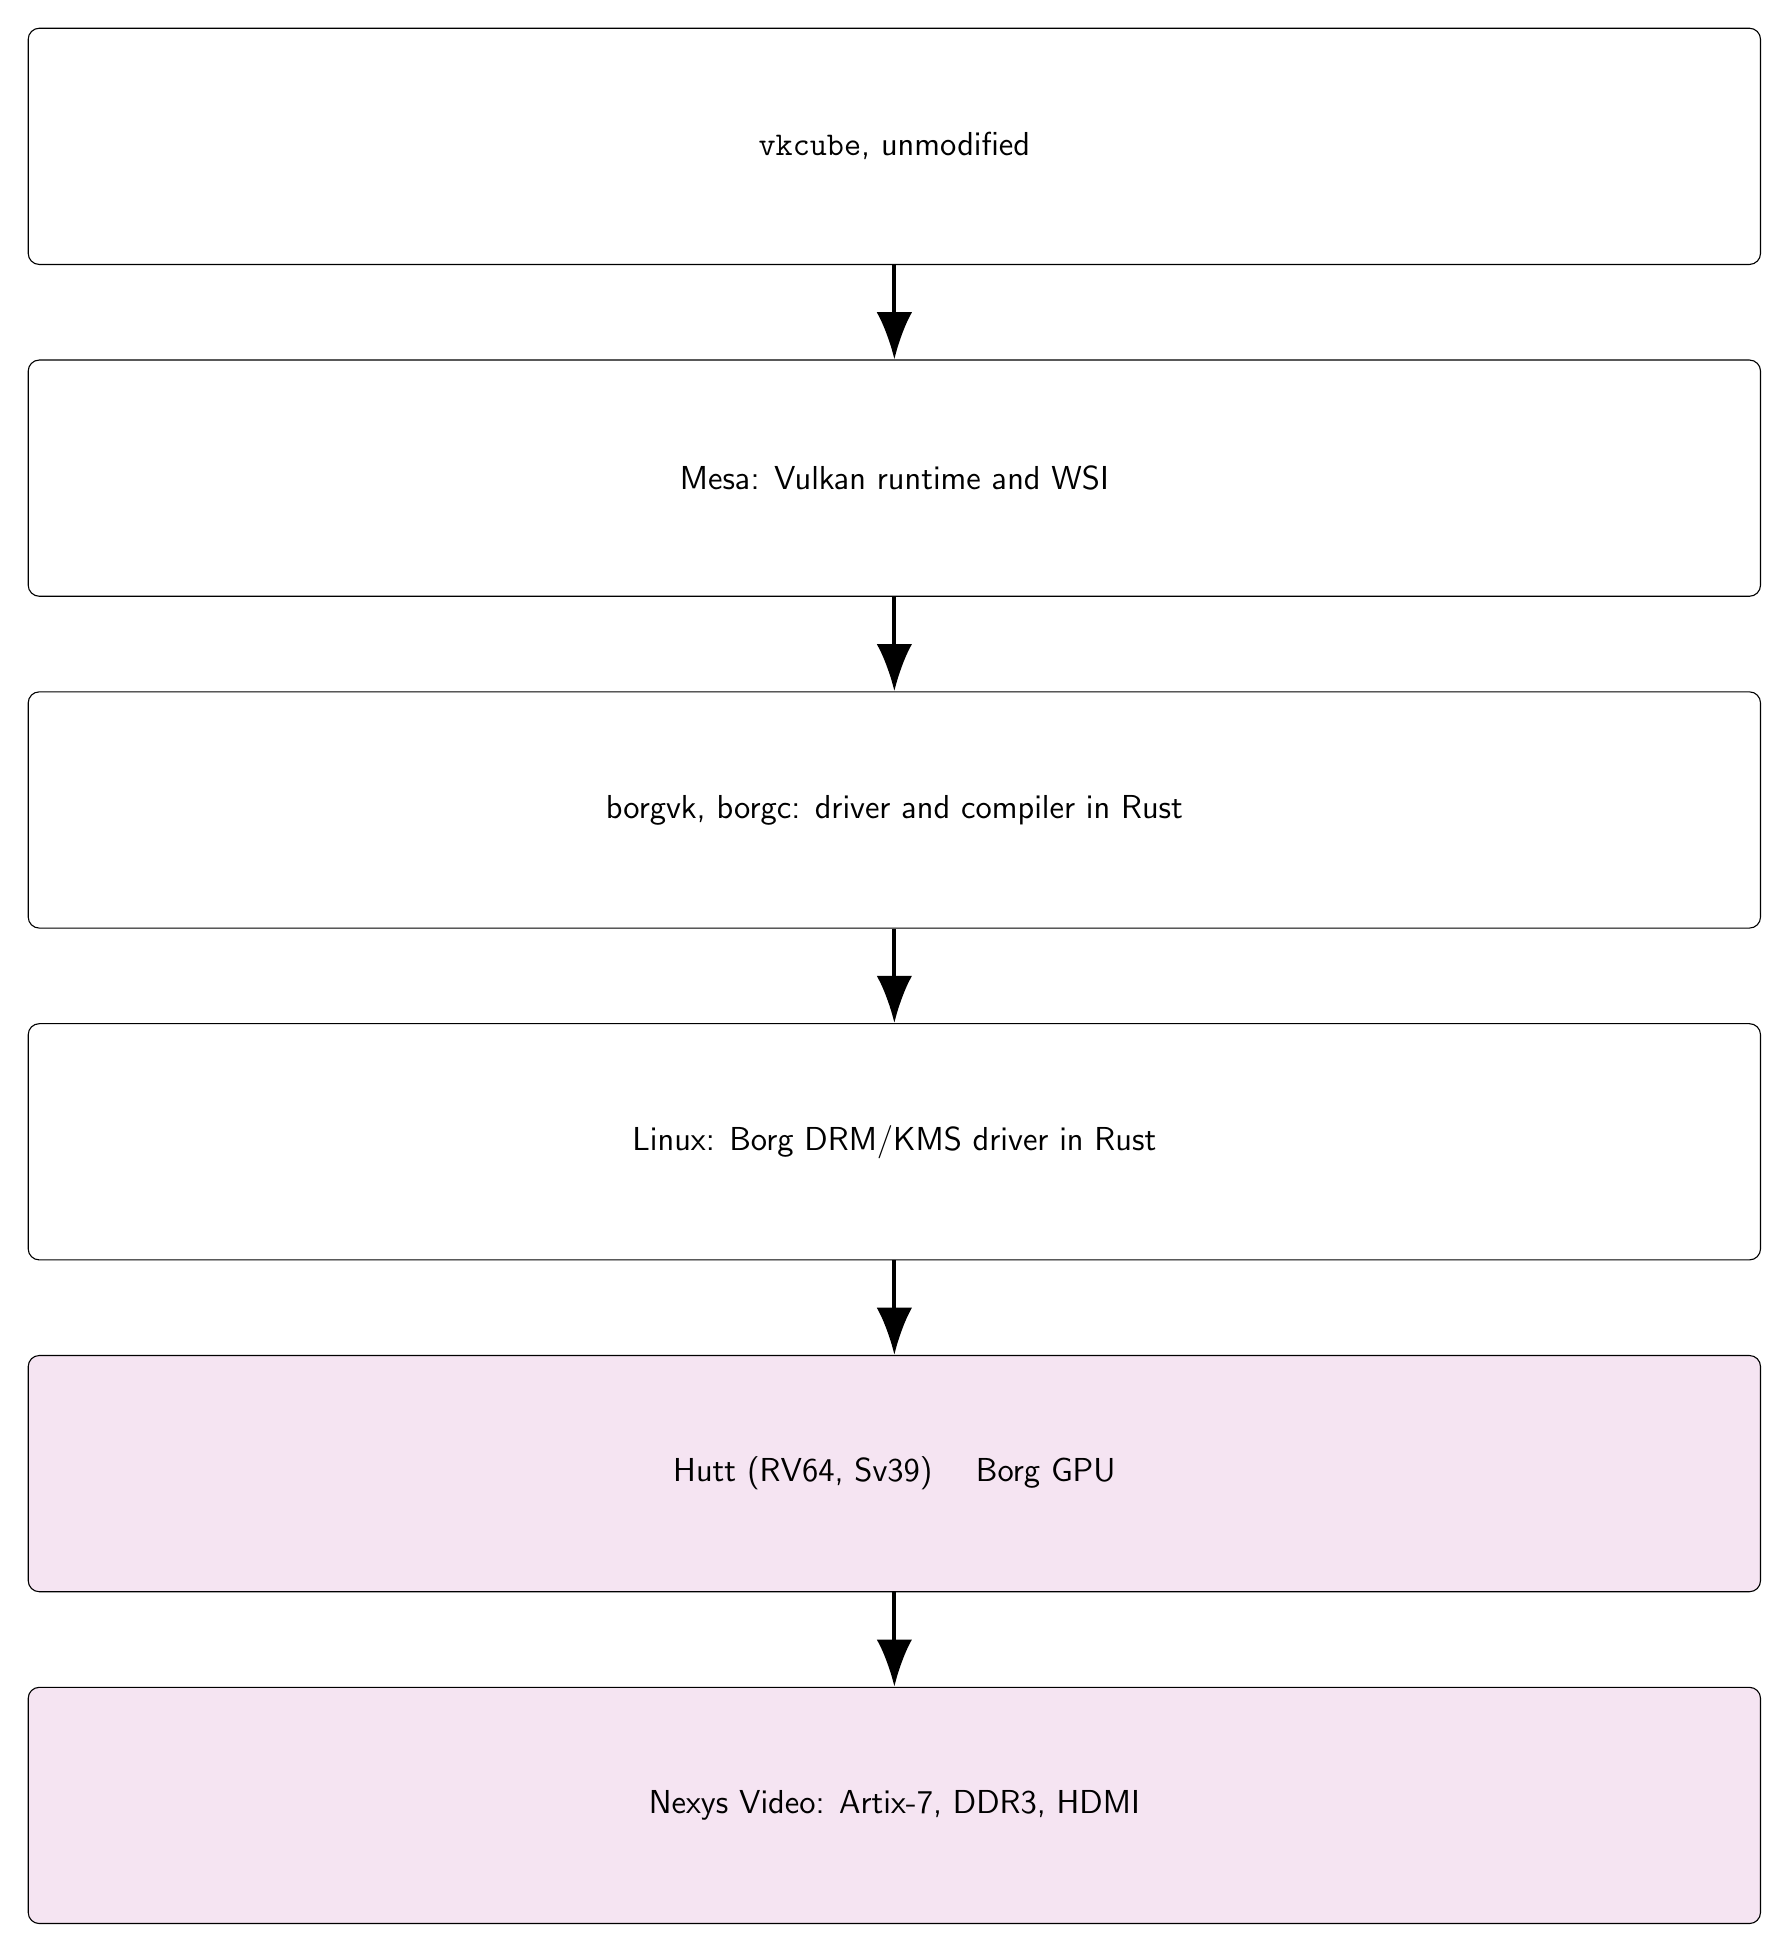
\begin{tikzpicture}[box/.style={draw, rounded corners=4pt, align=center, minimum height=30mm,
      minimum width=22cm, inner sep=8pt, fill=white, font=\large}, arr/.style={-{Latex[length=6mm]}, line width=1.5pt},
      hw/.style={box, fill=fosdem!12}]
    \node[box] (app) {\texttt{vkcube}, unmodified};
    \node[box, below=12mm of app] (mesa) {Mesa: Vulkan runtime and WSI};
    \node[box, below=12mm of mesa] (vk) {borgvk, borgc: driver and compiler in Rust};
    \node[box, below=12mm of vk] (krn) {Linux: Borg DRM/KMS driver in Rust};
    \node[hw, below=12mm of krn] (soc) {Hutt (RV64, Sv39) \quad Borg GPU};
    \node[hw, below=12mm of soc] (fpga) {Nexys Video: Artix-7, DDR3, HDMI};
    \foreach \a/\b in {app/mesa, mesa/vk, vk/krn, krn/soc, soc/fpga} \draw[arr] (\a) -- (\b);
  \end{tikzpicture}
}
\pblock{The hardware}{
  \begin{itemize}
    \item \textbf{Borg}, about 11,000 lines of Chisel: an FP32 shader core on 2x2 quads, a
      tile-based rasterizer, a texture unit with 51 formats, MSAA and compute.
    \item Its ISA is a RISC-V subset with the GPU instructions in the custom opcode space, all from
      one opcode file.
    \item \textbf{Hutt}, a small RV64 CPU with an MMU and caches, boots Linux.
    \item An early Borg is on a Tiny Tapeout chip (IHP), back in February 2027.
  \end{itemize}
}

\pblock{Open tools}{
  \begin{itemize}
    \item Chisel and CIRCT's \texttt{firtool} to Verilog; Verilator, arcilator and cocotb for
      simulation.
    \item Yosys and LibreLane for a GF180 chip.
    \item One Nix flake for the whole toolchain.
    \item The one closed tool: Vivado, for the Artix-7 bitstream.
  \end{itemize}
}
\column{0.333}
\pblock{Two drivers in Rust}{
  \textbf{borgvk}, a native Mesa Vulkan driver, about 12,400 lines of Rust. It started in C and
  moved to Rust step by step, working after every commit. Mesa's runtime does objects,
  synchronization and the window system.\\[5mm]
  \textbf{borgc} compiles NIR to Borg's ISA, about 7,500 lines of Rust: one instruction selector
  for graphics and compute. It refuses what it cannot compile instead of guessing.\\[5mm]
  \textbf{The kernel driver} is Rust too: register access checked against a map generated from the
  SystemRDL description, GEM buffer objects, and a KMS display with an fbdev console.
}
\pblock{How Borg draws a frame}{
  \centering
  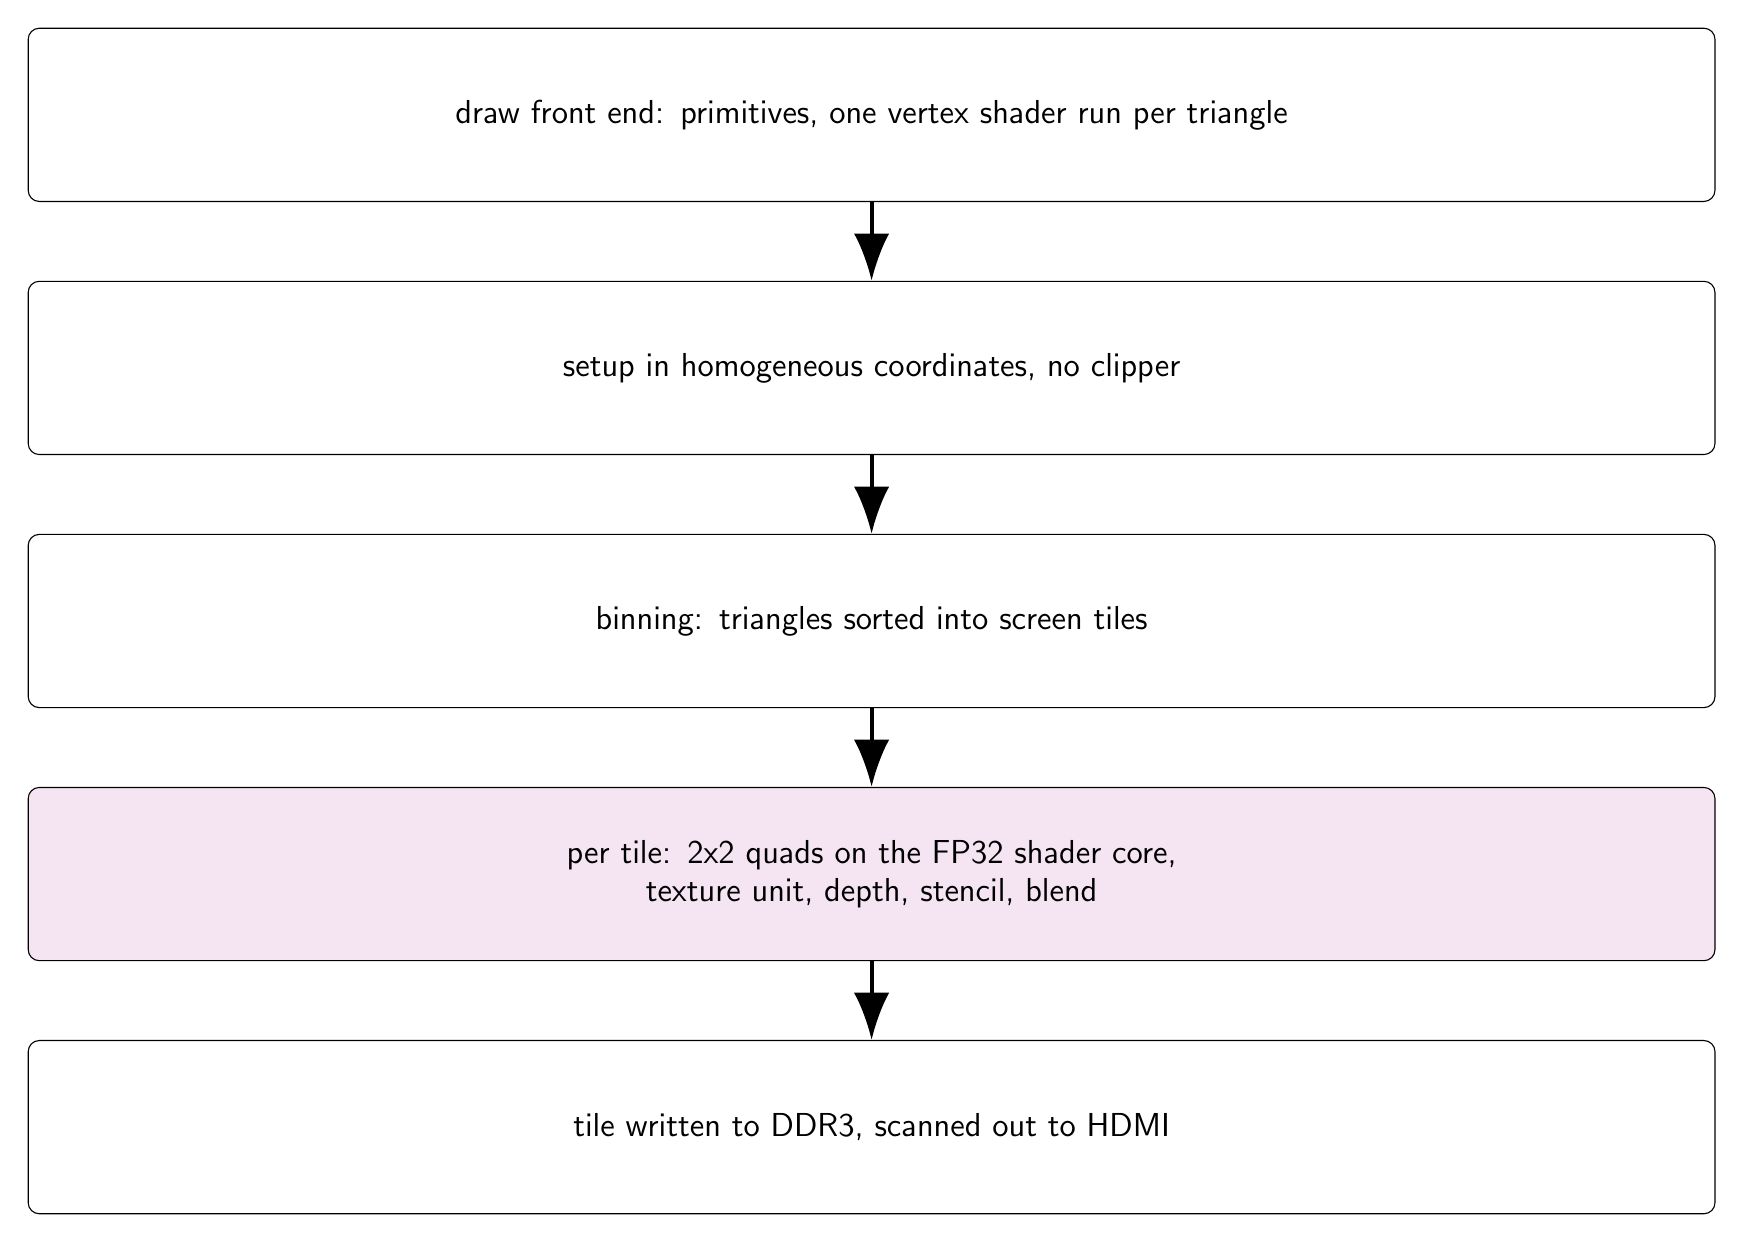
\begin{tikzpicture}[st/.style={draw, rounded corners=4pt, align=center, minimum height=22mm,
      text width=21cm, inner sep=6pt, fill=white, font=\large}, arr/.style={-{Latex[length=6mm]}, line width=1.5pt},
      tile/.style={st, fill=fosdem!12}]
    \node[st] (a) {draw front end: primitives, one vertex shader run per triangle};
    \node[st, below=10mm of a] (b) {setup in homogeneous coordinates, no clipper};
    \node[st, below=10mm of b] (c) {binning: triangles sorted into screen tiles};
    \node[tile, below=10mm of c] (d) {per tile: 2x2 quads on the FP32 shader core,\\texture unit, depth, stencil, blend};
    \node[st, below=10mm of d] (e) {tile written to DDR3, scanned out to HDMI};
    \foreach \x/\y in {a/b, b/c, c/d, d/e} \draw[arr] (\x) -- (\y);
  \end{tikzpicture}
}

\column{0.333}
\pblock{Tested like a GPU}{
  The Vulkan conformance tests run on the board, driven from a PC over USB, with the same command
  stream as under Linux. A simulator of the RTL, compiled with CIRCT's arcilator, is the debugger:
  board and simulator agree byte for byte on 825 recorded driver cases.
}
\pblock{Memory without copies}{
  Borg sees a 256 MB window of the DDR3. The kernel hands out buffer objects inside it, from a
  DMA pool in the device tree, each with its GPU address. borgvk uses buffers, images and render
  targets where they are.\\[5mm]
  No cache maintenance in software: Hutt's data cache writes through, and empties itself whenever
  Borg writes.
}
\pblock{Get involved}{
  \centering
  \qrcode[height=9cm]{https://github.com/gonsolo/Borg}\hspace{3cm}\qrcode[height=9cm]{https://gonsolo.github.io/Borg/}\\[3mm]
  code \hspace{10cm} book\\[6mm]
  \raggedright
  Everything is open source. Questions, ideas and patches welcome.
}
\end{columns}
\end{document}
